\section{The Gauss Map}
The Gauss map is deeply embedded in Minimal Surface Theory. This section requires knowledge of the preceding sections on Complex Analysis, Isothermal Parametrisation and the Weierstrass-Enneper Representation.

\subsection{Conformal Maps}
These are maps which preserve angle. A Linear transformation $T:\mathbb R^2 \rightarrow \mathbb R^2$ is conformal if, for fixed $\rho > 0$
\begin{displaymath}
T(\mathbf x) \cdot T(\mathbf y) = \rho^2 \mathbf x \cdot \mathbf y
\end{displaymath}

In relation to surfaces this implies that if a map between surfaces is conformal then the angles between tangent vectors are preserved through the map.

This can be seen from $\mathbf x \cdot \mathbf y = |\mathbf x||\mathbf y|\cos \theta$

\subsection{Tangent Vectors through the Gauss Map}
The Gauss map of a surface $M$ with parametrisation $\mathbf x(u,v)$ is a mapping from the surface to the unit sphere, denoted $G:M \rightarrow S^2$ and given by $G(p)=\mathbf N_p$ where $\mathbf N_p$ is the unit normal to M at p.

Now in order to see how angles are affected by the Gauss map we need to be able to transform tangent spaces through the Gauss map. The Gauss map as defined, takes a point p on the surface to a point q on $S^2$ via the unit normal to the surface. So if at point p we have a tangent plane, the unit normal is perpendicular to this; however due to the properties of the sphere the tangent plane at q on the sphere is also perpendicular to the same unit normal therefore the Gauss map, maps tangent planes onto themselves.

We can therefore write $G_*(\mathbf x_u)=N_u$ and $G_*(\mathbf x_v) = \mathbf N_v$



\subsection{Minimal iff Gauss Map Anti-Conformal}
\begin{theorem}
The Gauss Map of a surface M is Anti Conformal if and only if M is Minimal.
\label{GMAntiC}
\end{theorem}

\subsubsection{What does this mean?}
If we have a surface then we can find curves on the surface that intersect. If we use the Gauss map to take each point on the curves to a point on $S^2$ we get new curves on $S^2$.

By taking the tangent vectors at the points of intersection we can find the angle between the curves. If the angle between our original curves and our mapped curves is the same then the Gauss Map is said to be conformal for our surface.

Anti conformal simply means that while the angle between the curves is the same they've swapped orientation (eg instead of rotating curve 1 clockwise to get to curve 2, you now rotate curve 2 clockwise to get to curve 1.)

\subsubsection{Formulae required for the proof.}
Throughout we shall work in Isothermal Coordinates:
\begin{displaymath}
E=G \mbox{\ \ \ \ } F=0
\end{displaymath}
Also we need the basis expansion for the derivatives of the Gauss Map:

\begin{eqnarray}
\nonumber
G_*(\mathbf x_u) = \mathbf N_u &=& -\frac{L}{E} \mathbf x_u - \frac{M}{G} \mathbf x_v \\
G_*(\mathbf x_v) = \mathbf N_v &=& -\frac{M}{E} \mathbf x_u - \frac{N}{G} \mathbf x_v
\label{GMBE}
\end{eqnarray}

Lastly we need the formula for the Mean curvature of a surface parametrised by isothermal coordinates:

\begin{displaymath}
H = \frac{L+N}{2E} \mbox{\ \ \ } \left(\mbox {Eg \ } H=0 \Leftrightarrow L=-N \right)
\end{displaymath}

\subsubsection{Formal Proof}

\begin{prop}
Surface M, Minimal $\Rightarrow$ Gauss Map of M conformal.
\end{prop}

\begin{proof}

Need to show:
\begin{enumerate}
\item \begin{displaymath}
G_*(\mathbf x_u) \cdot G_*(\mathbf x_v) = \rho^2(u,v)\mathbf x_u \cdot \mathbf x_v
\end{displaymath}
\begin{eqnarray}
\nonumber
LHS &=& G_*(\mathbf x_u) \cdot G_*(\mathbf x_v) \\
\nonumber
&=& \mathbf N_u \cdot \mathbf N_v \\
\nonumber
&=& \left(-\frac{L}{E} \mathbf x_u - \frac{M}{E} \mathbf x_v \right) \cdot \left(-\frac{M}{E} \mathbf x_u - \frac{N}{E} \mathbf x_v \right) \\
\nonumber
&=& M\left(L+N\right) = 0 \mbox{\ \ \ \ \ since M minimal} \\
\nonumber
&=& \rho^2(u,v) G \mbox{\ \ \ \ \ Since G=0} \\
\nonumber
&=& \rho^2(u,v)\mathbf x_u \cdot \mathbf x_v = RHS
\end{eqnarray}   

\item \begin{displaymath}
G_*(\mathbf x_u) \cdot G_*(\mathbf x_u) = \rho^2(u,v)\mathbf x_u \cdot \mathbf x_u
\end{displaymath}
\begin{eqnarray}
\nonumber
G_*(\mathbf x_u) \cdot G_*(\mathbf x_u)&=& \mathbf N_u \cdot \mathbf N_u \\
\nonumber
&=& \left(-\frac{L}{E} \mathbf x_u - \frac{M}{E} \mathbf x_v \right) \cdot \left(-\frac{L}{E} \mathbf x_u - \frac{M}{E} \mathbf x_v \right) \\
\nonumber
&=& \frac{L^2}{E} + \frac{M^2}{E} = \rho^2 E
\end{eqnarray} 
\begin{displaymath}
\Leftrightarrow \rho^2 = \frac{L^2+M^2}{E^2}
\end{displaymath}

\item \begin{displaymath}
G_*(\mathbf x_v) \cdot G_*(\mathbf x_v) = \rho^2(u,v)\mathbf x_v \cdot \mathbf x_v
\end{displaymath}
\begin{eqnarray}
\nonumber
G_*(\mathbf x_v) \cdot G_*(\mathbf x_v) &=& \mathbf N_v \cdot \mathbf N_v \\
\nonumber
&=& \left(-\frac{M}{E} \mathbf x_u - \frac{N}{E} \mathbf x_v \right) \cdot \left(-\frac{M}{E} \mathbf x_u - \frac{N}{E} \mathbf x_v \right) \\
\nonumber
&=& \frac{M^2}{E} + \frac{N^2}{E} = \rho^2 E
\end{eqnarray} 
\begin{displaymath}
\Leftrightarrow \rho^2 = \frac{N^2+M^2}{E^2}
\end{displaymath}

\end{enumerate}

Since M is minimal we know $L = -N$, therefore $\rho^2$ is equal in (1), (2) and (3).
\end{proof}

\begin{prop}
Surface M has anti-conformal Gauss Map $\Rightarrow$ M Minimal.
\end{prop}

\begin{proof}
Gauss map is conformal so we know from the definition
\begin{displaymath}
G_*(\mathbf x_u) \cdot G_*(\mathbf x_v) = \rho^2(u,v)\mathbf x_u \cdot \mathbf x_v
\end{displaymath}

Remember we are working in isothermal coordinates so we have 
\begin{displaymath}F = \mathbf x_u \cdot \mathbf x_v = 0\end{displaymath}

\begin{displaymath}
\mathbf N_u \cdot \mathbf N_v = M(L+N) = 0
\end{displaymath}

So either L=-N in which case the surface is minimal and we are done or if this is not the case then we must have $M=0$.

Subbing $M=0$ into equations for $\mathbf N_u \cdot \mathbf N_u$ and $\mathbf N_v \cdot \mathbf N_v$ we know

\begin{eqnarray}
\nonumber
\mathbf N_u \cdot \mathbf N_u &=& \frac{L^2}{E} = \rho^2 E \\
\nonumber
\mathbf N_v \cdot \mathbf N_v &=& \frac{N^2}{E} = \rho^2 E
\end{eqnarray}

So

\begin{displaymath}
\frac{L^2}{E^2} = \rho^2 = \frac{N^2}{G^2} \Rightarrow \frac{L}{E} = \pm \frac{N}{G} 
\end{displaymath}

Setting $\frac{L}{E} = \frac{N}{G} = \kappa$ we can use the basis expansion (\ref{GMBE}) to write down the matrix for the differential of the Gauss Map for the two possibilities (e.g. the $\pm$).

\begin{displaymath}
\mathbf{dN_p} =
\left( \begin{array}{cc}
\kappa & 0 \\
0 & \pm \kappa
\end{array} \right)
\end{displaymath}

The principal curvatures are given by the determinant of $\mathbf{dN_p}$ so we have two cases:
\begin{enumerate} 
\item Principal curvatures $(\kappa, \kappa) \Rightarrow$ a Sphere (Note not anti conformal as this matrix does not reverse orientation).
\item Principal curvatures $(\kappa, -\kappa) \Rightarrow$ minimal surface ($H = \frac{\kappa_1 + \kappa_2}{2} = \frac{\kappa - \kappa}{2} = 0$) (Note anti conformal since this matrix reverses orientation!)
\end{enumerate}
\end{proof}

Putting these two directions together proves \ref{GMAntiC}.


\subsection{The Gauss Map in terms of the Weierstrass \\ Representation}

The Gauss Map is further linked to minimal surfaces through the Weierstrass-Enneper representation.
\begin{theorem}
Let M be a conformally parametrised surface with Weierstrass-Enneper representation (f,g). Then the Gauss map of M, $G: M \rightarrow \mathbb C \cup \left\{ \infty \right\}$, may be identified with the meromorphic function g.
\end{theorem}

In order to provide a proof we first need to introduce a parametrisation of the sphere (since the Gauss map maps our surface onto the sphere) known as Stereographic Projection.

\begin{definition}[Stereographic Projection]
Stereographic projection maps each point of the sphere onto the plane by projection from the North pole (N). This map is denoted by:

\begin{displaymath}
St: S^2/{N} \rightarrow \mathbb R^2
\end{displaymath}

and for the standard parametrisation of a sphere is defined by 

\begin{displaymath}
St(\cos u \cos v, \sin u \cos v, \sin v) = \left(\frac{\cos u \cos v}{1-\sin v}, \frac{\sin u \cos v}{1-\sin v}, 0 \right)
\end{displaymath}
\end{definition}

This becomes clear if we look at figure \ref{fig:stereographic}.

Furthermore as with the Gauss Map we can take the induced mapping on tangent vectors by differentiating with respect to u and v giving:

\begin{eqnarray}
\nonumber
St_*(\mathbf x_u) &=& \left(\frac{-\sin u \cos v}{1-\sin v},\frac{\cos u \cos v}{1-\sin v}, 0 \right) \\
\nonumber
St_*(\mathbf x_v) &=& \left(\frac{\cos u}{1-\sin v},\frac{\sin u}{1-\sin v}, 0 \right)
\end{eqnarray}

\begin{figure}[htbp]
	\centering
       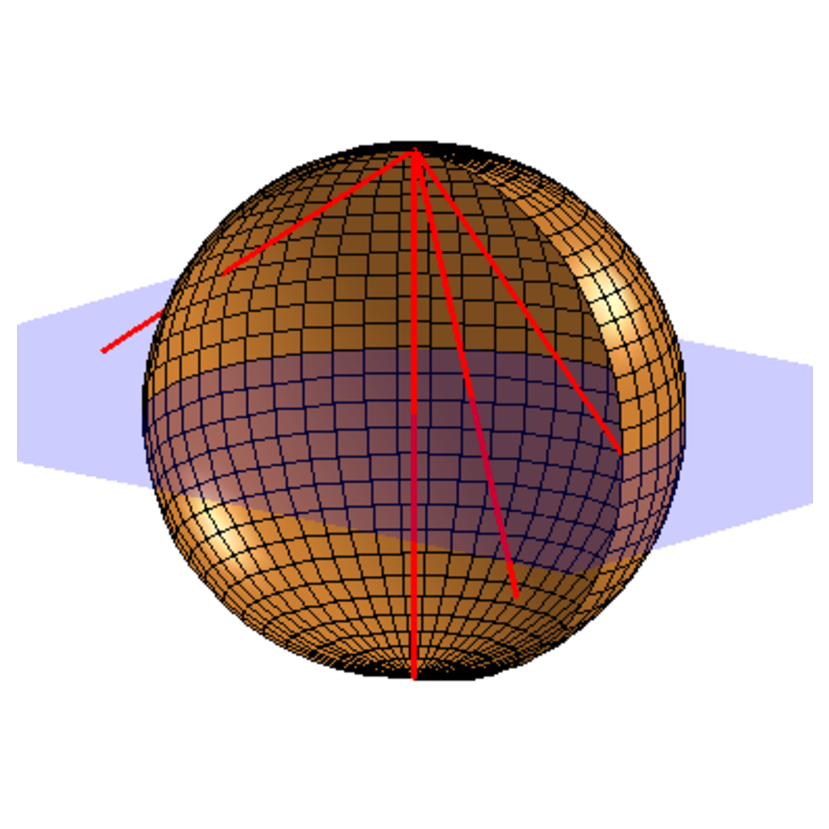
\includegraphics[width=8cm]{Images/Stereographic.eps}
   \caption{Stereographic Projection}
   \label{fig:stereographic}
\end{figure} 

\begin{proof}{(\cite{OPR} Page 92)}
From section \ref{WERep} recall that $\Phi = \frac{\partial \mathbf x}{\partial z}$, $\bar{\Phi} = \frac{\partial \mathbf x}{\partial \bar{z}}$ and

\begin{eqnarray}
\nonumber
\Phi^1 &=& \frac{1}{2}(1-g^2)f \\
\nonumber
\Phi^2 &=& \frac{i}{2}(1+g^2)f \\
\nonumber
\Phi^3 &=& fg\\
\end{eqnarray}

Our aim is to describe the Gauss map in terms of $\Phi^1$, $\Phi^2$ and $\Phi^3$

So take

\begin{eqnarray}
\nonumber
\mathbf x_u \times \mathbf x_v &=& ((\mathbf x_u \times \mathbf x_v)^1,(\mathbf x_u \times \mathbf x_v)^2,(\mathbf x_u \times \mathbf x_v)^3) \\
\nonumber
&=& (x_u^2x_v^3 - x_u^3x_v^2, x_u^3x_v^1-x^1_ux^3_v,x^1_ux^2_v-x^2_ux^1_v)
\end{eqnarray}

Taking the first component $(\mathbf x_u \times \mathbf x_v)^1 = x_u^2x_v^3 - x_u^3x_v^2$, (Recalling \ref{Phi}) we now write it in terms of components of $\Phi$.

\begin{eqnarray}
\nonumber
x_u^2x_v^3 - x_u^3x_v^2 &=& \Im[(x_u^2-ix_v^2)(x_u^3+ix_v^3)] \\
\nonumber 
&=& \Im\left[2\left(\frac{\partial x^2}{\partial z}\right)\cdot 2\left(\frac{\partial x^3}{\partial\bar{z}}\right)\right] \\
\nonumber
&=& 4 \Im(\Phi^2\bar{\Phi}^3)
\end{eqnarray} 
Following the same process we get
\begin{eqnarray}
\nonumber
(\mathbf x_u \times \mathbf x_v)^2 &=& 4 \Im(\Phi^3\bar{\Phi}^1) \\ 
\nonumber
(\mathbf x_u \times \mathbf x_v)^3 &=& 4 \Im(\Phi^1\bar{\Phi}^2)
\end{eqnarray}

And so we obtain
\begin{displaymath}
\mathbf x_u \times \mathbf x_v = 4 \Im(\Phi^2\bar{\Phi}^3,\Phi^3\bar{\Phi}^1,\Phi^1\bar{\Phi}^2) = 2(\Phi \times \bar{\Phi})
\end{displaymath}
since $z-\bar{z} = 2 \Im z$.

Now given that $\mathbf x(u,v)$ is isothermal

\begin{displaymath}
|\mathbf x_u \times \mathbf x_v| = |\mathbf x_u| \cdot |\mathbf x_v| = |\mathbf x_u|^2 = E = 2|\Phi|^2.
\end{displaymath}

Therefore

\begin{displaymath}
\mathbf N = \frac{\mathbf x_u \times \mathbf x_v}{|\mathbf x_u \times \mathbf x_v|} = \frac{2(\Phi \times \bar{\Phi})}{2|\Phi|^2} = \frac{\Phi \times \bar{\Phi}}{|\Phi|^2}
\end{displaymath}

We are now half way there, having written the unit normal in terms of $\Phi$.

Now using Stereographic projection we write the Gauss map $G:M\rightarrow \mathbb C \cup \infty$ in terms of the $\Phi^i$:

\begin{eqnarray}
\nonumber
G(\mathbf x(u,v)) &=& \mbox{St }(\mathbf N(u,v)) \\
\nonumber
&=& \mbox{St }\left(\frac{\Phi \times \bar{\Phi}}{|\Phi|^2}\right) \\
\nonumber
&=& \mbox{St }\left(\frac{2\Im(\Phi^2\bar{\Phi}^3,\Phi^3\bar{\Phi}^1,\Phi^1\bar{\Phi}^2)}{|\Phi|^2}\right) \\
\nonumber
&=& \left(\frac{2\Im(\Phi^2\bar{\Phi^3})}{|\Phi|^2-2\Im(\Phi^1\bar{\Phi}^2)}, \frac{2\Im(\Phi^3\bar{\Phi^1})}{|\Phi|^2-2\Im(\Phi^1\bar{\Phi}^2)}, 0 \right)
\end{eqnarray}

The last equality follows because

\begin{eqnarray}
\nonumber
\frac{x}{1-z} &=& \frac{2\Im(\Phi^2\bar{\Phi}^3)}{|\phi|^2}\cdot\frac{1}{1-\frac{2\Im(\Phi^2\bar{\Phi}^3)}{|\phi|^2}} \\
\nonumber
&=&\frac{2\Im(\Phi^2\bar{\Phi}^3)}{|\phi|^2}\cdot \frac{|\Phi|^2}{|\Phi|^2-2\Im(\Phi^1\bar{\Phi^2})} \\
\nonumber
&=& \frac{2\Im(\Phi^2\bar{\Phi^3})}{|\Phi|^2-2\Im(\Phi^1\bar\Phi^2)}
\end{eqnarray}
similarly for $\frac{y}{1-z}$. Identifying $(x,y) \in \mathbb R^2$ with $x+iy \in \mathbb C$ allows us to write
\begin{displaymath}
G(\mathbf x(u,v)) = \frac{2\Im(\Phi^2\bar{\Phi}^3)+2i\Im(\Phi^3\bar{Phi}^1)}{|\Phi|^2-2\Im(\Phi^1\bar{\Phi}^2)}
\end{displaymath}

Now, considering the numerator $N$ of this fraction:

\begin{eqnarray}
\nonumber
N &=& 2\Im(\Phi^2\bar{Phi}^3) + 2i\Im(\Phi^3\bar{Phi}^1) \\
\nonumber
&=& \frac{1}{i}[\Phi^2\bar{Phi}^3-\bar{\Phi}^2\Phi^3+i\Phi^3\bar{Phi}^1-i\bar{\Phi}^3\Phi^1] \\
\nonumber
&=& \Phi^3(\bar{\Phi}^1+i\bar{\Phi}^2)-\bar{\Phi}^3(\Phi^1+i\Phi^2)
\end{eqnarray}

Also
\begin{displaymath}
0 = (\Phi)^2 =(\Phi^1)^2+(\Phi^2)^2+(\Phi^3)^2 = (\Phi^1-i\Phi^2)(\Phi^1+i\Phi^2)+(\Phi^3)^2
\end{displaymath}
so
\begin{displaymath}
\Phi^1 + i \Phi^2 =\frac{-(\Phi^3)^2}{\Phi^1-i\Phi^2}
\end{displaymath}

Then we have
\begin{eqnarray}
\nonumber
N &=& \Phi^3(\bar{\Phi}^1+i\bar{\Phi}^2)+\bar{\Phi}^3\frac{(\Phi^3)^2}{\Phi^1-i\Phi^2} \\
\nonumber
&=&\frac{\Phi^3[(\Phi^1-i\Phi^2)(\bar{\Phi}^1+i\bar{\Phi}^2)+|\Phi^3|^2]}{\Phi^1-i\Phi^2} \\
\nonumber
&=& \frac{\Phi^3}{\Phi^1-i\Phi^2}[|\Phi^1|^2+|\Phi^2|^2+|\Phi^3|^2 + i(\bar{\Phi}^2\phi^1-\Phi^2\bar{\Phi}^1)] \\
\nonumber
&=& \frac{\Phi^3}{\Phi^1-i\Phi^2} [|\Phi|^2 - 2\Im(\Phi^1\bar{\Phi}^2)]
\end{eqnarray}

The second factor of the numerator $N$ cancels the denominator of $G(\mathbf x(u,v))$, and we end up with

\begin{displaymath}
G(\mathbf x(u,v))=\frac{\Phi^3}{\Phi^1-i\Phi^2}
\end{displaymath}

Which is our definition for $g(z)$ (given in Section \ref{WERep}) as required.
\end{proof}